\begin{figure*}[t!]
  \centering
  \begin{subfigure}{0.24\textwidth}
    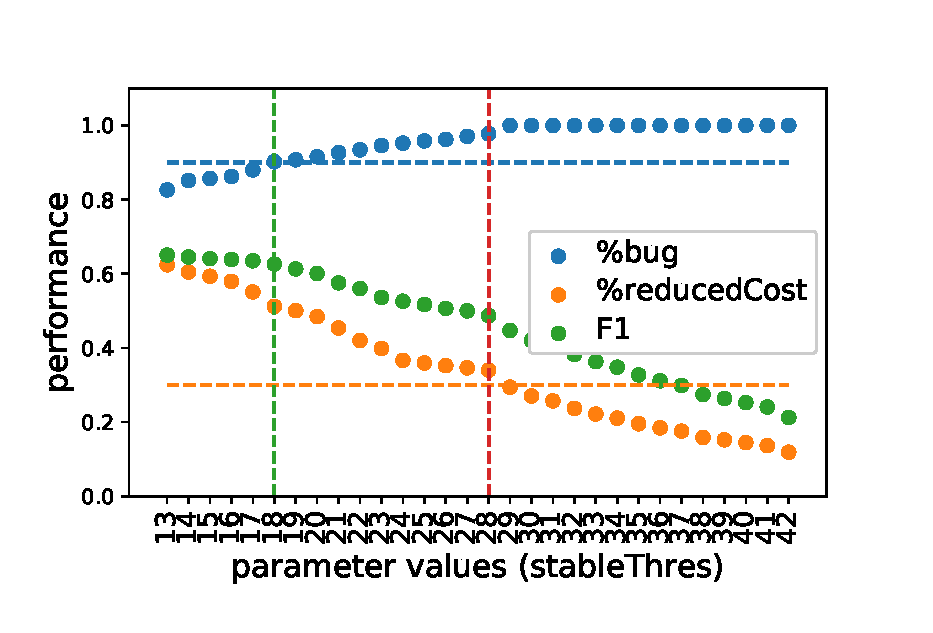
\includegraphics[width=4.8cm]{figure/threLearningTrend.eps}
	 \caption{Trend}
	 \label{fig:TLTrend}
  \end{subfigure}
  \begin{subfigure}{0.24\textwidth}
    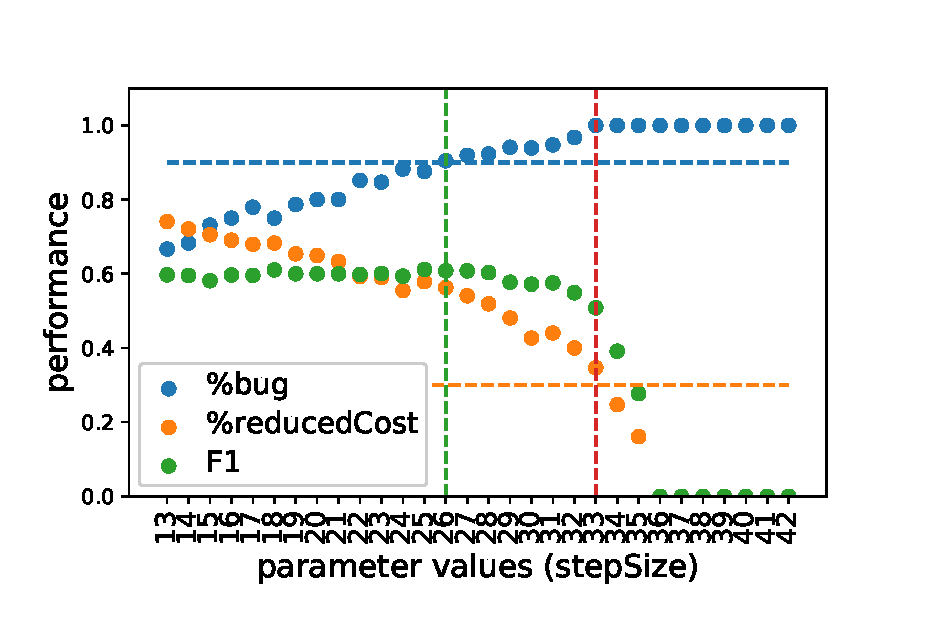
\includegraphics[width=4.8cm]{figure/threLearningArrival.eps}
	\caption{Peak}
   \label{fig:TLArrival}
  \end{subfigure}
  \begin{subfigure}{0.24\textwidth}
    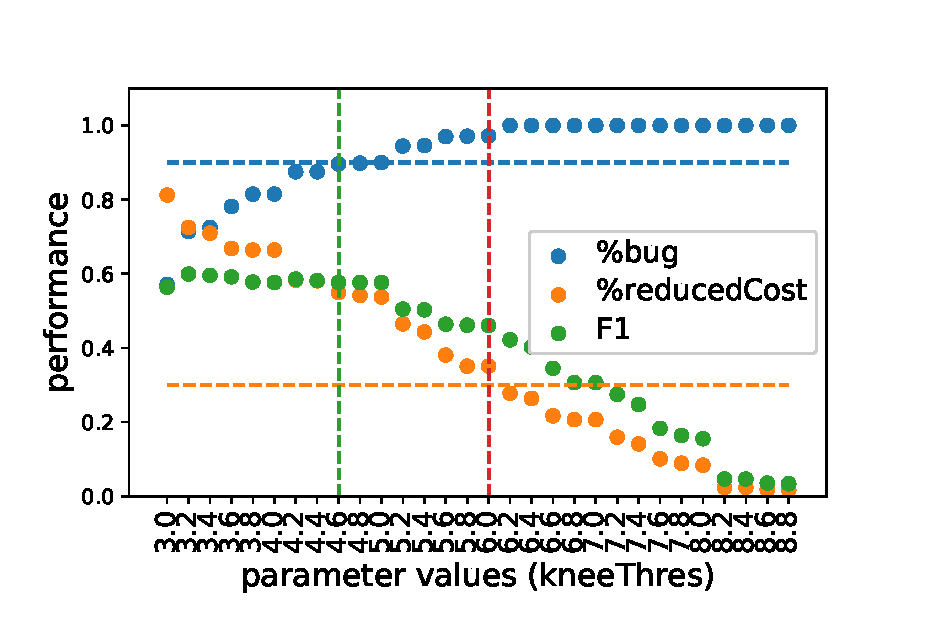
\includegraphics[width=4.8cm]{figure/threLearningKnee.eps}
	\caption{Knee}
    \label{fig:TLKnee}
  \end{subfigure}
   \begin{subfigure}{0.24\textwidth}
    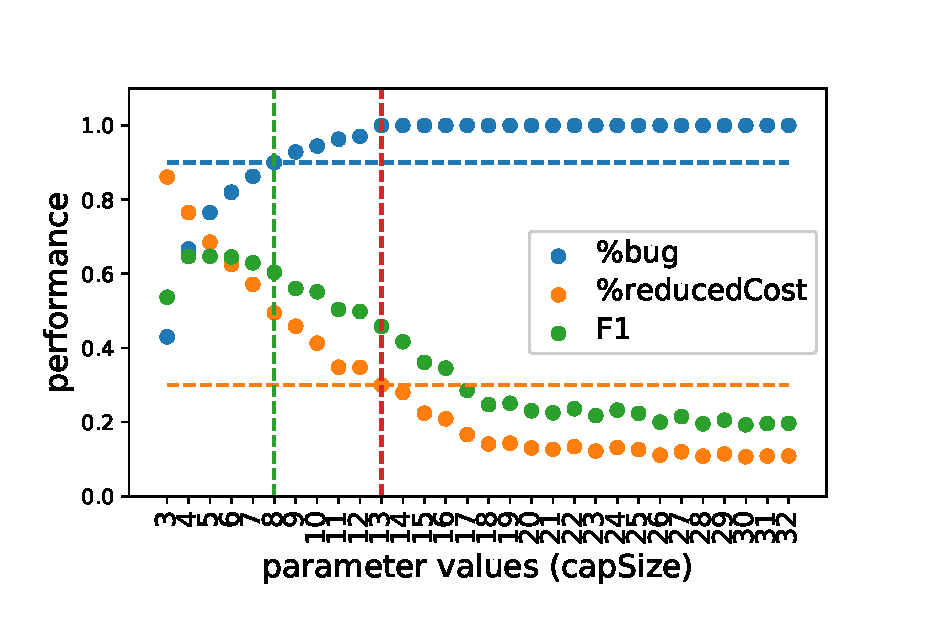
\includegraphics[width=4.8cm]{figure/threLearningM0.eps}
	\caption{M0}
    \label{fig:TLM0}
  \end{subfigure}
   \begin{subfigure}{0.24\textwidth}
    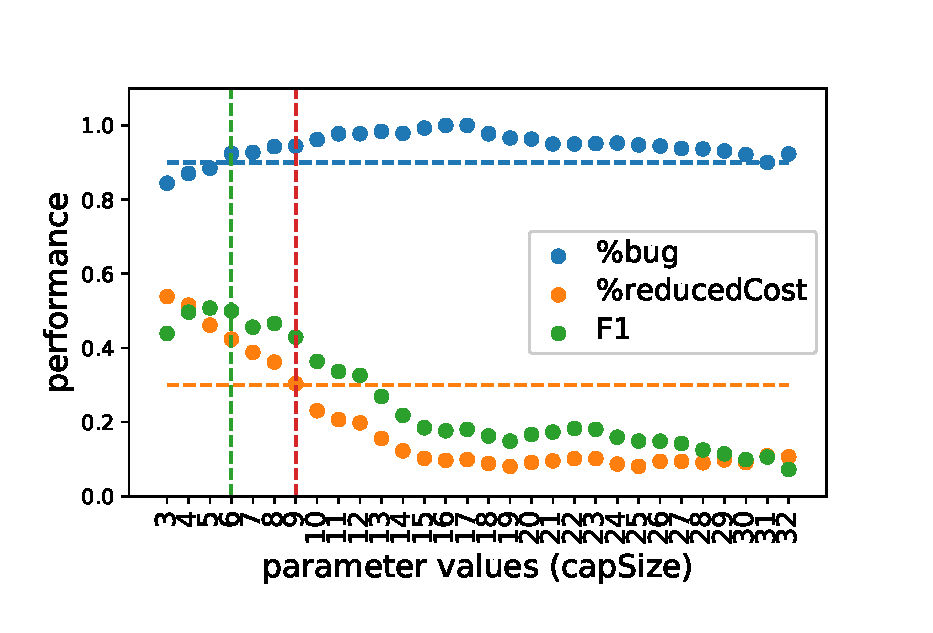
\includegraphics[width=4.8cm]{figure/threLearningMth.eps}
	 \caption{Mth}
	 \label{fig:TLMth}
  \end{subfigure}
  \begin{subfigure}{0.24\textwidth}
    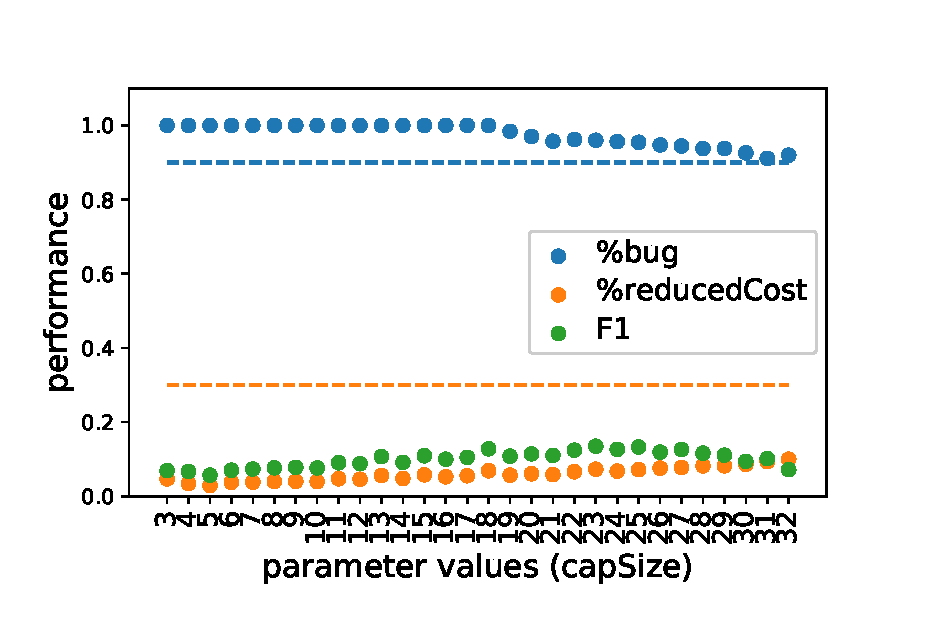
\includegraphics[width=4.8cm]{figure/threLearningMhJK.eps}
	\caption{MhJK}
   \label{fig:TLMhJK}
  \end{subfigure}
  \begin{subfigure}{0.24\textwidth}
    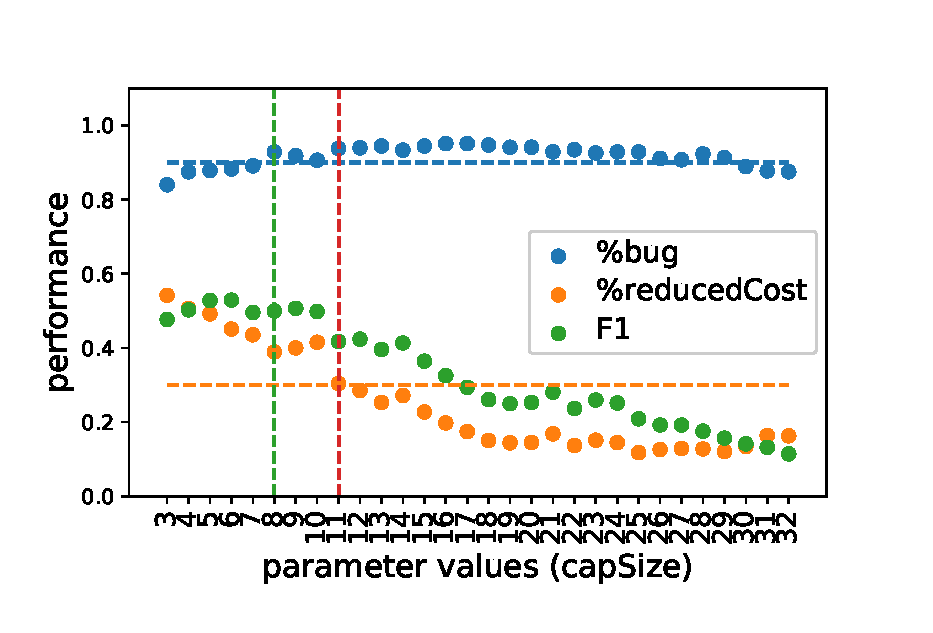
\includegraphics[width=4.8cm]{figure/threLearningMhCH.eps}
	\caption{MhCH}
    \label{fig:TLMhCh}
  \end{subfigure}
   \begin{subfigure}{0.24\textwidth}
    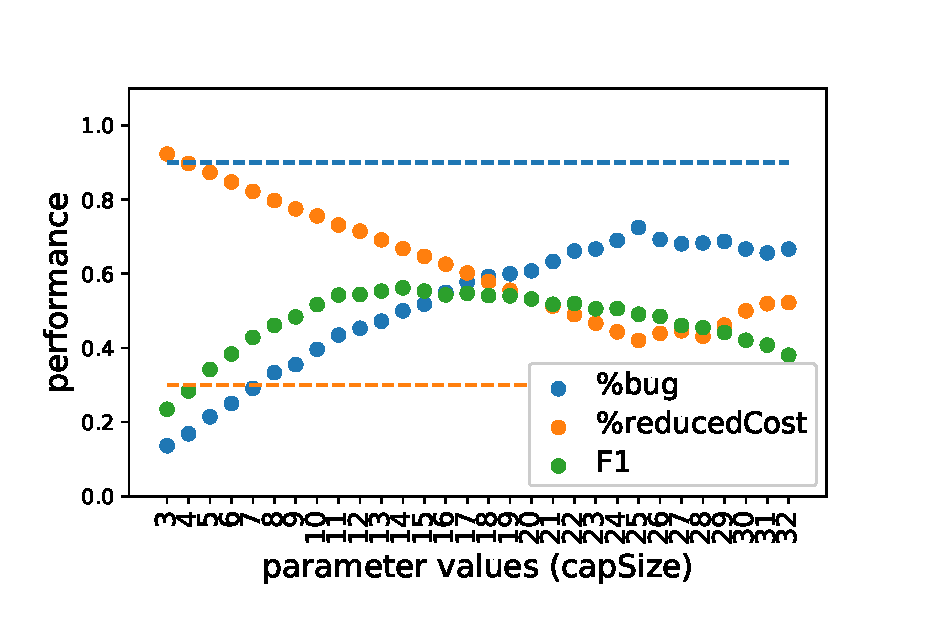
\includegraphics[width=4.8cm]{figure/threLearningMtCH.eps}
	\caption{MtCH}
    \label{fig:TLMtCh}
  \end{subfigure}
  \caption{Influence of parameter values on prediction performance, i.e., sensitivity analysis (RQ1)}
  \label{fig:thres}
% \vspace{-0.1in}
\end{figure*}


